\documentclass[12pt, twoside, openright]{report}

%%%%%%%%%%%%%%%%%%%%%%%%%%%%%%%%%%%%%%%%%%%%%%%%%%%%%%%%%%%%%%%%%%%%%%%%%%%%%%%%%%
%%%%%%%%%%%%%%%%%%%%%%%%%%%%%%%%%%% PACKAGES %%%%%%%%%%%%%%%%%%%%%%%%%%%%%%%%%%%%%
%%%%%%%%%%%%%%%%%%%%%%%%%%%%%%%%%%%%%%%%%%%%%%%%%%%%%%%%%%%%%%%%%%%%%%%%%%%%%%%%%%

\usepackage{color}
% REMEMBER TO ADD OFFSET FOR BINDING!!!!
\usepackage[a4paper,width=170mm,top=25mm,bottom=25mm,bindingoffset=0mm]{geometry}
\usepackage{fancyhdr}
\usepackage[protrusion=true,expansion=true]{microtype}
\usepackage{titling}
\usepackage{titlesec}
\usepackage{hyperref}
\usepackage{changepage}
\usepackage{graphicx}
\graphicspath{ {images/} }
\usepackage{ifthen}
\usepackage{etoolbox}
\usepackage{wrapfig}
\usepackage{musicography}
\usepackage{graphbox}
\usepackage{tabu}
\usepackage{amsmath}
\usepackage{amssymb}
\usepackage{xfrac}
\usepackage[english]{babel}

%%%%%%%%%%%%%%%%%%%%%%%%%%%%%%%%%%%%%%%%%%%%%%%%%%%%%%%%%%%%%%%%%%%%%%%%%%%%%%%%%%
%%%%%%%%%%%%%%%%%%%%%%%%%%%%%%%%% SPECIFIC INFO %%%%%%%%%%%%%%%%%%%%%%%%%%%%%%%%%%
%%%%%%%%%%%%%%%%%%%%%%%%%%%%%%%%%%%%%%%%%%%%%%%%%%%%%%%%%%%%%%%%%%%%%%%%%%%%%%%%%%

\title{Pitch Correction}
\author{Walter Smuts}

\newcounter{quoteCounter}
\setcounter{quoteCounter}{1}
\newcommand\addQuote{
\begin{center}

	\ifnum\thequoteCounter=1
		In the beginning the Universe was created.\\
		This has made a lot of people very angry and has\\
		been widely regarded as a bad move.\\
		\vspace{1cm}
		- Douglas Adams
	\fi

	\ifnum\thequoteCounter=2
		Always remember that you are absolutely unique.\\
		Just like everyone else.\\
		\vspace{1cm}
		- Margaret Mead
	\fi

	\ifnum\thequoteCounter=3
		Talking about music\\
		is like dancing about architecture.\\
		\vspace{1cm}
		 — Steve Martin
	\fi


	\ifnum\thequoteCounter=4
		Wagner’s music is better than it sounds.\\
		\vspace{1cm}
		— Mark Twain
	\fi

	\ifnum\thequoteCounter=5
		A gentleman is someone who can\\
		play the accordion,
		but doesn't.\\
		\vspace{1cm}
		— Tom Waits
	\fi

	\ifnum\thequoteCounter=6
		I'd agree with you, but then\\
		we'd both be wrong.\\
		\vspace{1cm}
		- Russell Lynes
	\fi

	\stepcounter{quoteCounter}

	\ifnum\thequoteCounter=7
		\setcounter{quoteCounter}{1}
	\fi

\end{center}

}

%%%%%%%%%%%%%%%%%%%%%%%%%%%%%%%%%%%%%%%%%%%%%%%%%%%%%%%%%%%%%%%%%%%%%%%%%%%%%%%%%%
%%%%%%%%%%%%%%%%%%%%%%%%%%%%% SECTION HEADING STYLES %%%%%%%%%%%%%%%%%%%%%%%%%%%%%
%%%%%%%%%%%%%%%%%%%%%%%%%%%%%%%%%%%%%%%%%%%%%%%%%%%%%%%%%%%%%%%%%%%%%%%%%%%%%%%%%%

% Chapter style
\titleformat{\chapter}
{\normalfont \LARGE \bfseries}
{}
{0em}
{\MakeUppercase}
[\titlerule \ifthenelse{\equal{\thechapter}{0}}{}{ \small\it \chaptertitlename \space \thechapter}]

% Chapter spacing
\titlespacing*{\chapter}
  {0pt}
  {15pt}
  {25pt}

\patchcmd{\thebibliography}{\chapter*{\bibname}}
{\cleardoublepage\MakeUppercase
{\vspace*{1cm}\hspace{-7mm} \normalfont \LARGE \bfseries References}

\vspace{2.5mm}
\titlerule\thispagestyle{plain}
}
{}{}

%%%%%%%%%%%%%%%%%%%%%%%%%%%%%%%%%%%%%%%%%%%%%%%%%%%%%%%%%%%%%%%%%%%%%%%%%%%%%%%%%%
%%%%%%%%%%%%%%%%%%%%%%%%%%%%%%%%%% PAGE STYLES %%%%%%%%%%%%%%%%%%%%%%%%%%%%%%%%%%%
%%%%%%%%%%%%%%%%%%%%%%%%%%%%%%%%%%%%%%%%%%%%%%%%%%%%%%%%%%%%%%%%%%%%%%%%%%%%%%%%%%

% Page layout
\pagestyle{fancy}

% Front page offset
\makeatletter
\if@twoside
	\newcommand{\frontpageoffset}{-1.5cm}
\else

	\newcommand{\frontpageoffset}{0cm}
\fi
\makeatother

% Offset to force numbers to margins
\newcommand{\numberoffset}{\hspace{-1cm}}

% Assuming odd pages are right and even are left pages
% Chapter Pages
\fancypagestyle{plain}{
	\fancyhead{}
	\makeatletter
	\if@twoside
		\fancyhf{}
		\fancyfoot[LE,RO]{\thepage\numberoffset}
	\fi
	\makeatother
	\renewcommand{\headrulewidth}{0pt}
}

% Redefine clear double page to leave an empty page
\makeatletter
\def\cleardoublepage{\clearpage\if@twoside \ifodd\c@page\else
\hbox{}
\vspace*{\fill}
\begin{center}
	\it \addQuote
\end{center}
\vspace{\fill}
\thispagestyle{empty}
\newpage
\if@twocolumn\hbox{}\newpage\fi\fi\fi}
\makeatother

%%%%%%%%%%%%%%%%%%%%%%%%%%%%%%%%%%%%%%%%%%%%%%%%%%%%%%%%%%%%%%%%%%%%%%%%%%%%%%%%%%
%%%%%%%%%%%%%%%%%%%%%%%%%%%% PAGE HEADERS AND FOOTERS %%%%%%%%%%%%%%%%%%%%%%%%%%%%
%%%%%%%%%%%%%%%%%%%%%%%%%%%%%%%%%%%%%%%%%%%%%%%%%%%%%%%%%%%%%%%%%%%%%%%%%%%%%%%%%%

% General Header
\fancyhead{}
\fancyhead[LE,RO]{\nouppercase\leftmark}
\fancyhead[LO,RE]{\TITLE}

% General Footer
\fancyfoot{}
\makeatletter
\if@twoside
	\fancyfoot[LE]{\numberoffset\thepage}
	\fancyfoot[RO]{\thepage\numberoffset}
\else
	\fancyfoot[C]{\thepage}
\fi
\makeatother
%%%%%%%%%%%%%%%%%%%%%%%%%%%%%%%%%%%%%%%%%%%%%%%%%%%%%%%%%%%%%%%%%%%%%%%%%%%%%%%%%%
%%%%%%%%%%%%%%%%%%%%%%%%%%%%%%% START OF DOCUMENT %%%%%%%%%%%%%%%%%%%%%%%%%%%%%%%%
%%%%%%%%%%%%%%%%%%%%%%%%%%%%%%%%%%%%%%%%%%%%%%%%%%%%%%%%%%%%%%%%%%%%%%%%%%%%%%%%%%

\begin{document}

% Save title
\makeatletter
\let\TITLE\@title
\makeatother

% First page
\begin{titlepage}
\begin{adjustwidth*}{}{\frontpageoffset} % For centering front page
\begin{center}
	\vspace*{4cm}

	{\Huge\textbf\thetitle}

	{\it of digital audio}

	\vspace{0.8cm}
	
\includegraphics[width=0.4\textwidth]{UCT.jpg}
	\vspace{0.8cm}

	by \theauthor
	\vspace{0.8cm}

	Prepared for Associate Professor Fred Nicolls\\
	Department of Electrical Engineering\\
	University of Cape Town\\
	South Africa\\
	\vspace{2cm}
	\today
\end{center}
\end{adjustwidth*}
\end{titlepage}
\cleardoublepage

% Reset page numbering and use roman numerals
\pagenumbering{roman}
\setcounter{page}{1}

\null
\vfill

\section*{\center Abstract}
\thispagestyle{plain}

This thesis investigates the design, implementation and testing of a pitch
correction system in the context of digital audio. A modular design is proposed
which contains a frequency detection module and a frequency scaling module.
Testing metrics are designed to evaluate the performance of the system as a whole
as well as individual modules separately. The algorithms implemented and tested
for the frequency detection module are the zero-crossing method and
autocorrelation method. For the frequency scaling module a simple overlap and add
method was tested a swell as the phase vocoder approach. The combination that
produces the best results is the \color{red}winning combo\color{black}.

\vfill
\vfill

\newpage
\null
\vfill

\section*{\center Declaration}
\thispagestyle{plain}

I declate that:
\vspace{3mm}
\hrule
\begin{enumerate}
\item
I know that plagiarism is wrong. Plagiarism is to use another’s work and
pretend that it is one’s own.
\item
I have used the IEEE convention for citation and referencing. Each contribution
to, and quotation in, this report from the work(s) of other people has been
attributed, and has been cited and referenced.
\item
This report is my own work.
\item
I have not allowed, and will not allow, anyone to copy my work with the
intention of passing it off as his or her own work.
\end{enumerate}

\begin{tabular}{ l l }
 Name: &  Walter Smuts\\
 Date: & \today
\end{tabular}
\vspace{3mm}
\hrule
\vspace{3mm}

\includegraphics[width=2cm]{Signature.png}
\par {\it Signature}

\vfill
\vfill

\tableofcontents
\thispagestyle{plain}

%%%%%%%%%%%%%%%%%%%%%%%%%%%%%%%%%%%%%%%%%%%%%%%%%%%%%%%%%%%%%%%%%%%%%%%%%%%%%%%%%%
%%%%%%%%%%%%%%%%%%%%%%%%%%%%%%% START OF CHAPTERS %%%%%%%%%%%%%%%%%%%%%%%%%%%%%%%%
%%%%%%%%%%%%%%%%%%%%%%%%%%%%%%%%%%%%%%%%%%%%%%%%%%%%%%%%%%%%%%%%%%%%%%%%%%%%%%%%%%

\chapter{Introduction}
% Reset page numbering and to Arabic numbers
\setcounter{page}{1}
\pagenumbering{arabic}
% !tex root = ../Thesis.tex

\section{Problem Statement}

\color{red}
To Do:
\begin{itemize}
	\item Describe what pitch correction is
	\item Describe why it is difficult
	\begin{itemize}
		\item Pitch detection is not trivial
		\item Why you can't just speed up sound and slow it down
		\item Convey the essence of the problem
	\end{itemize}
		\item Motivate why it's needed
		\begin{itemize}
		\item One small out of tune note causes a whole new re-recording
		\item Quick fix after recording
		\item Live performers can now sing
		\item Produces a quirky robotic effect that can be desirable
		\item Case against audio pitch correction
		\begin{itemize}
			\item Less freedom to professional singers
			\item Vibrato, colour etc
			\item Conceals talent
		\end{itemize}
		\item Biggest case for: Interesting mathematical project
	\end{itemize}
\end{itemize}
\color{black}

\section{History of Audio Pitch Correction}

One of the first occurrences of pitch manipulation in music, at least the first
occurrence that was found by the author, was of a song called ``The Chipmunk
Song'' from the animated music group ``Alvin and the Chipmunks''. The goal was to
raise the pitch of the voice of a singer to sound an octave higher than his actual
voice. This was accomplished by recording the song at half the wanted tempo and
playing back the recording at twice the speed when mixing. The technology used in
audio recordings was still analog tape recordings and the whole process was done
using these tapes. The effect of speeding up a recording to achieve a pitch
shift became known as the ``Chipmunk Effect''. The approach earned the group two
Grammy awards in 1958.

In 1977 Eventide introduced a new product, the Eventide H949 Harmonizer, capable
of incremental pitch shifting. This was sold as a ``de-glitch pitch shifter'' and
was intended to be used to fix intonation errors and add harmonization effects
after recording. Other features commonly used was to stretch the time of radio
recordings of advertisements to be an exact duration without affecting the pitch.
The pitch shifting was implemented using single side-band modulation
techniques and was done digitally.

\begin{figure}[h]
	\centering
	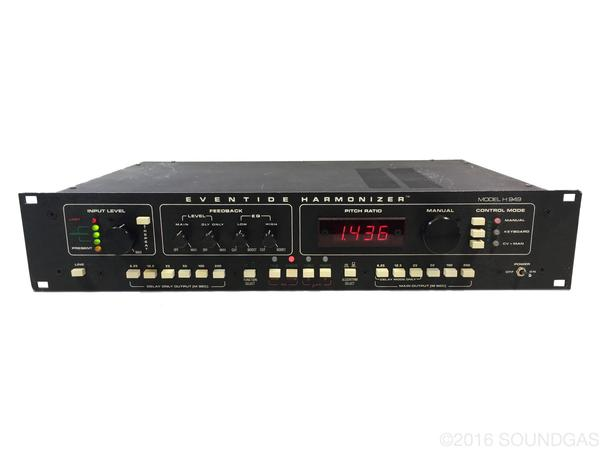
\includegraphics[width=0.9\textwidth,trim={0mm 55mm 0mm 55mm},clip]
	{EventideH949}
	\caption{Eventide H949 Harmonizer Rack Mounted Unit}
	\label{fig:EventideH949}
\end{figure}

In 1996 Andy Hildebrand, an electrical engineer, was investigating seismic data
when he realised that the same techniques he was using to investigate the data
could be used to alter the pitch of audio files. His techniques for detecting
pitch, using a simplification of the autocorrelation function, was considered
superior to the state of the art at that time. He implemented the first version of
his pitch correcting algorithm on his Macintosh computer. His first demonstration
was considered a success and the company ``Antares Audio'' was founded. They
created a product called ``AutoTune'' which was popularised in 1998 by Cher in her
song ``Believe''.

\begin{figure}[h]
	\centering
	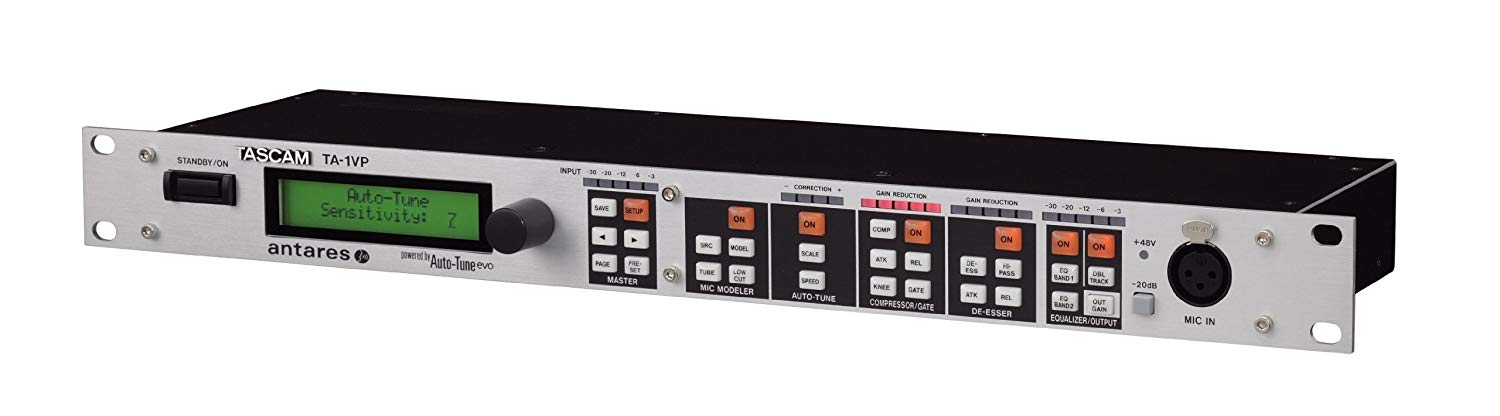
\includegraphics[width=0.9\textwidth,trim={30mm 20mm 30mm 30mm},clip]
	{AutoTuneRack}
	\caption{AutoTune Rack Mounted Unit}
	\label{fig:AutoTuneRack}
\end{figure}

AutoTune comes in a rack mounted unit for live performances shown in figure
\ref{fig:AutoTuneRack} or as a plugin with the interface shown in figure
\ref{fig:AutoTunePlugin}. The software has evolved to allow for many more features
than the original pitch correction effect that the name suggests. Modern AutoTune
is still considered the state of the art product by audio engineers.

\color{red}
To Do:
\begin{itemize}
	\item Open source pitch correction AutoTalent by Tom Baran
	\item Smule App
\end{itemize}
\color{black}

\section{Approach Taken}

\color{red}
To Do:
\begin{itemize}
	\item Discuss structure of report
	\item Show final implementation
	\item Summarise results and conclusion section
\end{itemize}
\color{black}


\chapter{Literature Review}
% !tex root = ../Thesis.tex

This literature review attempts to cover all the subjects relevant to pitch
correction. Music theory is investigated first, covering the topics of human
pitch perception and tuning. This section attempts to determine what it means for
pitch to be correct and how this relates to frequency. The idea is to get a list of
correct frequencies derived from a tuning system. After it is well known what
is musically considered to be a correct pitch, the general structure of how pitch
correction is approached is investigated. This structure naturally splits up into
modules and each of these modules is investigated further.

\section{Music Theory}

The intent of this section is to come up with a definition of what will be
considered correct pitch. Some foundational work is required to define basic
musical concepts in a rigorous way. To start we need to define exactly what is
meant by a musical note.

A note is a sound made from a musical instrument. It has a pitch, volume, timbre
and length. These are the characteristics a musician would consider when composing
a piece of music. Each of these characteristics have a more rigorous scientific
counterpart they are related to. Pitch relates to frequency; Volume relates to
amplitude; timbre relates to harmonic content and length relates to duration. The
characteristic pair relevant to pitch correction is the pitch and frequency pair
and needs to be covered in more depth.

\begin{wrapfigure}{L}{0.5\textwidth}
\includegraphics[width=0.5\textwidth,trim={3mm 0mm 20mm 8mm},clip]{Frequency-Vs-Pitch}
\caption{"Frequency vs Pitch"}
\label{fig:FrequencyVsPitch}
\end{wrapfigure}

Pitch and frequency are terms often used interchangeably but does not refer to the
same concept. Pitch is a \textit{sensation} experienced by humans when they hear
notes containing frequencies between 31Hz and 17.6 kHz\cite{Hearing}. The
sensation of pitch is scaled on an subjective ``high'' and ``low'' scale. The
higher the frequency, the higher the pitch perceived and the lower the frequency,
the lower the pitch perceived. This relationship between pitch and frequency is
generally considered to be logarithmic. Slight deviations from the expected
logarithmic relationship was found \cite{PitchVsFrequency} but was deemed minor
and unnecessary to incorporate for this project.

In Figure \ref{fig:FrequencyVsPitch} the relationship of frequency and pitch is
shown. Pitch is generally denoted by letters ranging from A to G with
sharps(\musSharp) and flats(\musFlat) called accidentals.  This is due to a long
history of convention and is irrelevant for now. The main takeaway is that the
perceived change in pitch is constant for each successive note. From this graph it
can be seen that frequency is exponentially dependent on pitch, or inversely,
pitch is logarithmically dependent on frequency.

\color{red}
To do:
\begin{itemize}
	\item In tune
	\item Harmony
	\item Tuning system and equal tempered tuning
	\item Tie back to the fact that this gives us a definition of correct
\end{itemize}
\color{black}

\section{General Pitch Correction Structure}

\color{red}
To Do:
\begin{itemize}
	\item Stages and sections needed e.g.:
	\begin{itemize}
		\item Segmentation/Windowing
		\item Frequency detection
		\item Decide where to shift
		\item Frequency scaling
	\end{itemize}
	\item Add a flow diagram
\end{itemize}
\color{black}

\section{Segmentation}

\color{red}
To do:
\begin{itemize}
	\item Describe what segmentation is and why it is necessary
	\item Describe stages
	\begin{itemize}
		\item Split (overlap)
		\item Do computation
		\item Stitch (overlap and add)
	\end{itemize}
	\item Reason to overlap and size of overlapping (TRADE-OFF)
	\item Window size (TRADE-OFF)
	\begin{itemize}
		\item Small means low resolution
		\item Large means latency
		\item Small generally means more computation
	\end{itemize}
	\item Properties to preserve relevant to real time auto tuning
\end{itemize}
\color{black}

\section{Frequency Detection}

\color{red}
To do:
\begin{itemize}
	\item Explain that there is no single go-to method
	\item Different methods have different characteristics
	\item What is important for this application
	\item Give overview of which methods will be investigated
\end{itemize}
\color{black}

\subsection{Zero Crossing Method}

\color{red}
To do:
\begin{itemize}
	\item Describe method roughly
	\item More in depth description comes in implementation section
\end{itemize}
\color{black}

\subsection{Periodogram Method}

\color{red}
To do:
\begin{itemize}
	\item Describe method roughly
	\item More in depth description comes in implementation section
\end{itemize}
\color{black}

\subsection{Max FFT Method}

\color{red}
To do:
\begin{itemize}
	\item Describe method roughly
	\item More in depth description comes in implementation section
\end{itemize}
\color{black}

\subsection{YIN's Method}

\color{red}
To do:
\begin{itemize}
	\item Describe method roughly
	\item More in depth description comes in implementation section
\end{itemize}
\color{black}

\section{Frequency Scaling}

\color{red}
To do:
\begin{itemize}
	\item General approach is to expand/extrapolate frequency
	\item Time domain approaches and frequency domain approaches
	\item Introduce two approaches Phase Vocoder and pitch synchronous overlap and add
\end{itemize}
\color{black}

\subsection{Phase Vocoder}

\color{red}
To do:
\begin{itemize}
	\item Describe method roughly
	\item More in depth description comes in implementation section
\end{itemize}
\color{black}

\subsection{PSOLA}

\color{red}
To do:
\begin{itemize}
	\item Describe method roughly
	\item More in depth description comes in implementation section
\end{itemize}
\color{black}


\chapter{Implementation}
% !tex root = ../Thesis.tex

This chapter describes the design, module implemetation and final implemetations
of the pitch correction system. Since one of the goals of this report is to
compare the performance of using different modules, the evaluation metrics used
are described first. Theses metrics are described first to reflect the fact that
the metrics were designed before the structure and submodules were implemented in
an effort to minimise biased results. Once these metrics are well understood, the
desing and implementation of the pitch corrector and it's submodules are
described.

\section{Evaluation Metrics}

The goal of the metrics described below is to give a meaningful quantitative way
of measuring the success of the pitch corrector. It's a way to compare the
performance of different sub modules and choose the configuration that produces
the best result. Since the ultimate goal of an audio pitch corrector is to produce
better sounding music, the most rigorous way to judge the effectiveness of the
pitch corrector would be to run a psychological survey on which combination of sub
modules sound best. This is beyond the scope of this project. Instead, some
simplifications are made and metrics are designed based on the research done on
music theory. These metrics act as a proxy for the results given by a
physiological survey and are much easier and cheaper to run. Two aspects of the
pitch corrector are chosen to be assessed.  The effectiveness of it and the noise
or distortion of the audio signal introduced by the pitch corrector.

\color{red}
To Do:
\begin{itemize}
	\item Maybe describe the properties metrics should have
\end{itemize}
\color{black}

The effectiveness metric is a way of measuring how much the pitch corrector
corrects the pitch.

\color{red}
To Do:
\begin{itemize}
	\item Describe effectiveness metric further
\end{itemize}
\color{black}

The effectiveness metric unfortunately relies on the frequency detector to be
absolutely correct. This is because it depends on the results of the frequency
contour before the correction was mad and after the correction was made. Therefore
a separate metric is designed to evaluate the frequency detector as an individual
module.  This is to provide some confidence that the frequency detector module
does provide a reasonably good approximation for the actual frequency contour.

\color{red}
To Do:
\begin{itemize}
	\item Describe Frequency Detection Metric
	\item Describe noise metric
	\item Describe why a frequency scaling metric is also needed
	\item Describe Frequency Scaling metric
	\item Summarise all the metrics (in a table?)
\end{itemize}
\color{black}

\section{Pitch Correction Design}

\color{red}
To do:
\begin{itemize}
	\item Touch on subsections and why each needs a section
\end{itemize}
\color{black}

\subsection{Structure}

\color{red}
To do:
\begin{itemize}
	\item Segmentation!!!
	\begin{itemize}
		\item Describe what segmentation is and why it is necessary
		\item Describe stages
		\begin{itemize}
			\item Split (overlap)
			\item Do computation
			\item Stitch (overlap and add)
		\end{itemize}
		\item Reason to overlap and size of overlapping (TRADE-OFF)
		\item Window size (TRADE-OFF)
		\begin{itemize}
			\item Small means low resolution
			\item Large means latency
			\item Small generally means more computation
		\end{itemize}
		\item Properties to preserve relevant to real time auto tuning
	\end{itemize}
	\item Flow diagram
	\item Actual code snips from Octave source code
\end{itemize}
\color{black}

\subsection{Interface}

\color{red}
To do:
\begin{itemize}
	\item Interface philosophy
	\item Frequency detectors and scalers should be swappable
\end{itemize}
\color{black}

\section{Choosing Wanted Frequency}

\color{red}
To do:
\begin{itemize}
	\item Describe why choosing wanted frequency is not trivial
	\item Naive approach
	\begin{itemize}
		\item Describe approach
		\item Show results of approach
	\end{itemize}
	\item Schmitt Trigger Approach
	\begin{itemize}
		\item Describe approach
		\item Show results of approach
	\end{itemize}
	\item Evaluation Metric
	\begin{itemize}
		\item Describe metric
		\item Show why Schmitt trigger is better
	\end{itemize}
\end{itemize}
\color{black}

\section{Frequency Detector}

\color{red}
To do:
\begin{itemize}
	\item Explain that this is the basis for the frequency scaler
	\item Explain other things
\end{itemize}
\color{black}

\subsection{Zero Crossing Method}

\color{red}
To do:
\begin{itemize}
	\item Describe method in more detail than lit review
	\item Show snips of code and graphically what it's doing
	\item Show performance metrics
\end{itemize}
\color{black}

\subsection{Autocorrelation Method}

\color{red}
To do:
\begin{itemize}
	\item Describe method in more detail than lit review
	\item Show snips of code and graphically what it's doing
	\item Show performance metrics
\end{itemize}
\color{black}

\section{Frequency Scaler}

\color{red}
To do:
\begin{itemize}
	\item Explain time vs frequency approaches
	\item Explain other things
\end{itemize}
\color{black}

\subsection{Phase Vocoder}

\color{red}
To do:
\begin{itemize}
	\item Describe method in more detail than lit review
	\item Show snips of code and graphically what it's doing
	\item Show performance metrics
\end{itemize}
\color{black}

\subsection{Simple Overlap and Add}

\color{red}
To do:
\begin{itemize}
	\item Describe method in more detail than lit review
	\item Show snips of code and graphically what it's doing
	\item Show performance metrics
\end{itemize}
\color{black}

\section{Pitch Corrector}

\color{red}
To do:
\begin{itemize}
	\item Describe which modules were added put together
	\item Describe why each module was chosen
	\item Describe each system and show its performance
\end{itemize}
\color{black}

\section{Concept Expansion}

\color{red}
To do:
\begin{itemize}
	\item Explain that more cool stuff were found
	\item Post Correction
	\item Harmonization
	\item Pitch Scaling by a Constant Factor
\end{itemize}
\color{black}


\chapter{Results}
% !tex root = ../Thesis.tex

In this chapter, the results of metrics designed for the frequency detector and
pitch correction system will be given and interpreted. The frequency detector will
be discussed first and the pitch correction system will follow. Some real vocal
recordings will also be corrected using a few different configurations of the
pitch correction system. This is to give some confidence that the system can hadle
real data and doesn't just rely on clean signals the metrics have been designed
for. These examples are not rigorous by nature and should just be considered as a
final real world demonstaration.

\section{Frequency Detector}

The noise robustness metric for each of the two pitch detection algorithms were
run. This checks how much noise can be introduced into a signal with a known pitch
contour before the pitch detector produces unacceptable results. Unacceptable is
seen as having a mean squared pitch error of more than $0.59\times10^-6$. The
metric will be quoted in decibels of noise.

Figure \ref{fig:NoiseRobustnessZCM} shows a graph plotting the square pitch error,
of the Zero Crossing frequency detector, as a function of additive noise in
decibels. The square pitch error is plotted using $log_{10}$ scaling to make the
graph more readable.

\begin{figure}[h]
	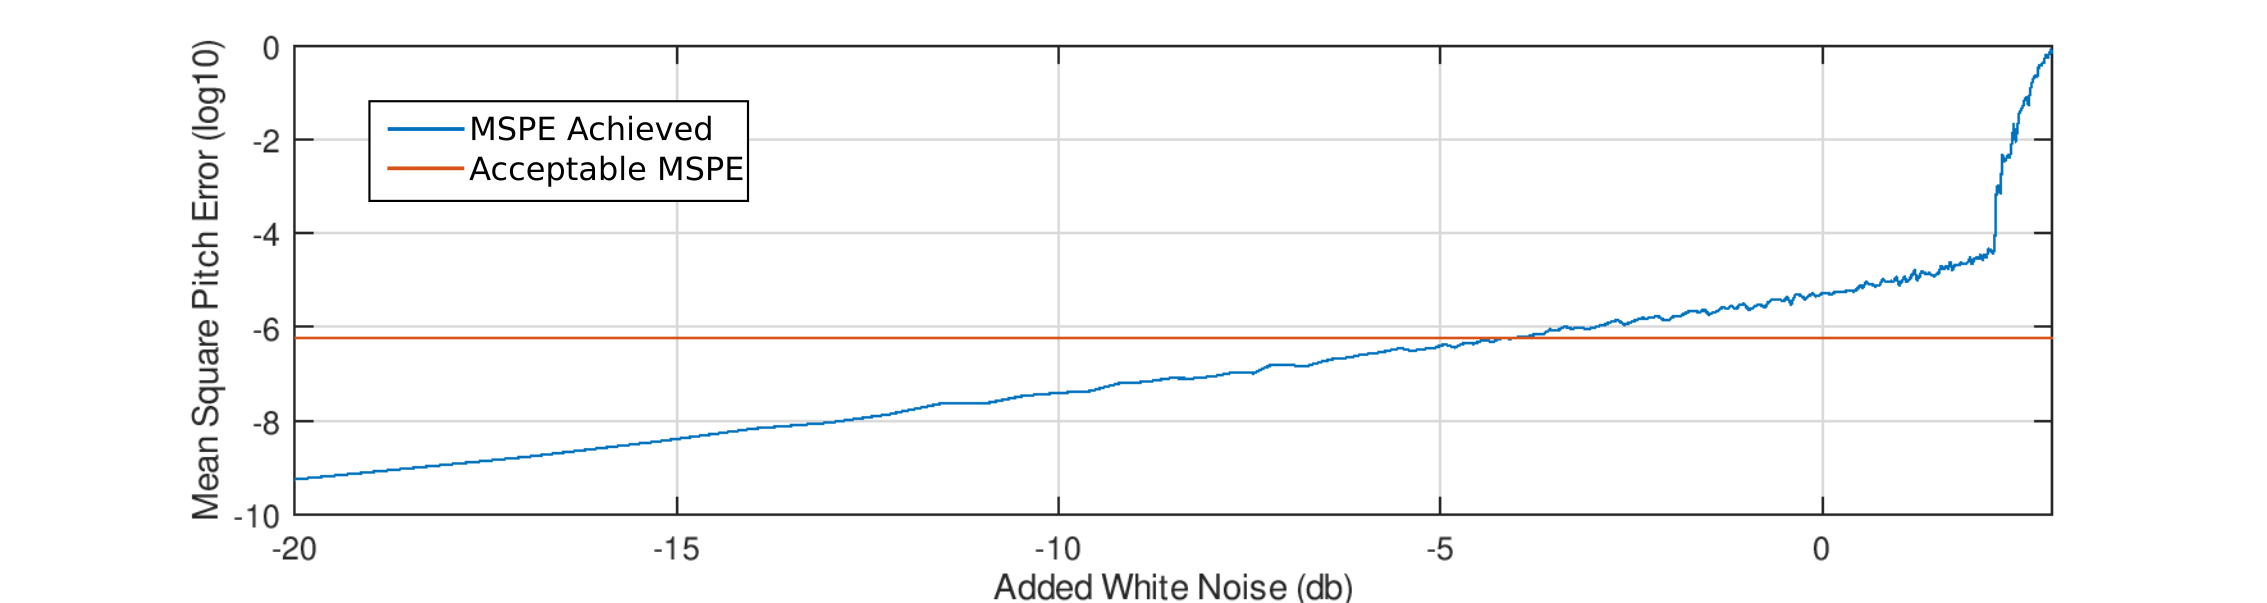
\includegraphics[width=\textwidth,trim={2.5cm 0mm 2.5cm 0mm},clip]
	{NoiseRobustnessZCM}
	\caption{Zero Crossing Method Noise Robustness}
	\label{fig:NoiseRobustnessZCM}
\end{figure}

Since the input signal has an amplitude of 0 decibel, the signal to noise ratio
can easily be determined. The graph shows that the zero crossing method requires a
SNR of 4.5db in order to function at a acceptable level.

Figure \ref{fig:NoiseRobustnessAutoCorr} shows a similar graph but of the
autocorrelation method. The SNR required for acceptable performance is 17.8db.
This is worse than the expected and indicates an error in implementation. It is
postulated that this is a resolution error and oversampling of the signal before
autocorrelation is required. It is also worth mentioning that very little time was
spent inspecting the autocorrelation code and that mistakes are highly likely.

\begin{figure}[h]
	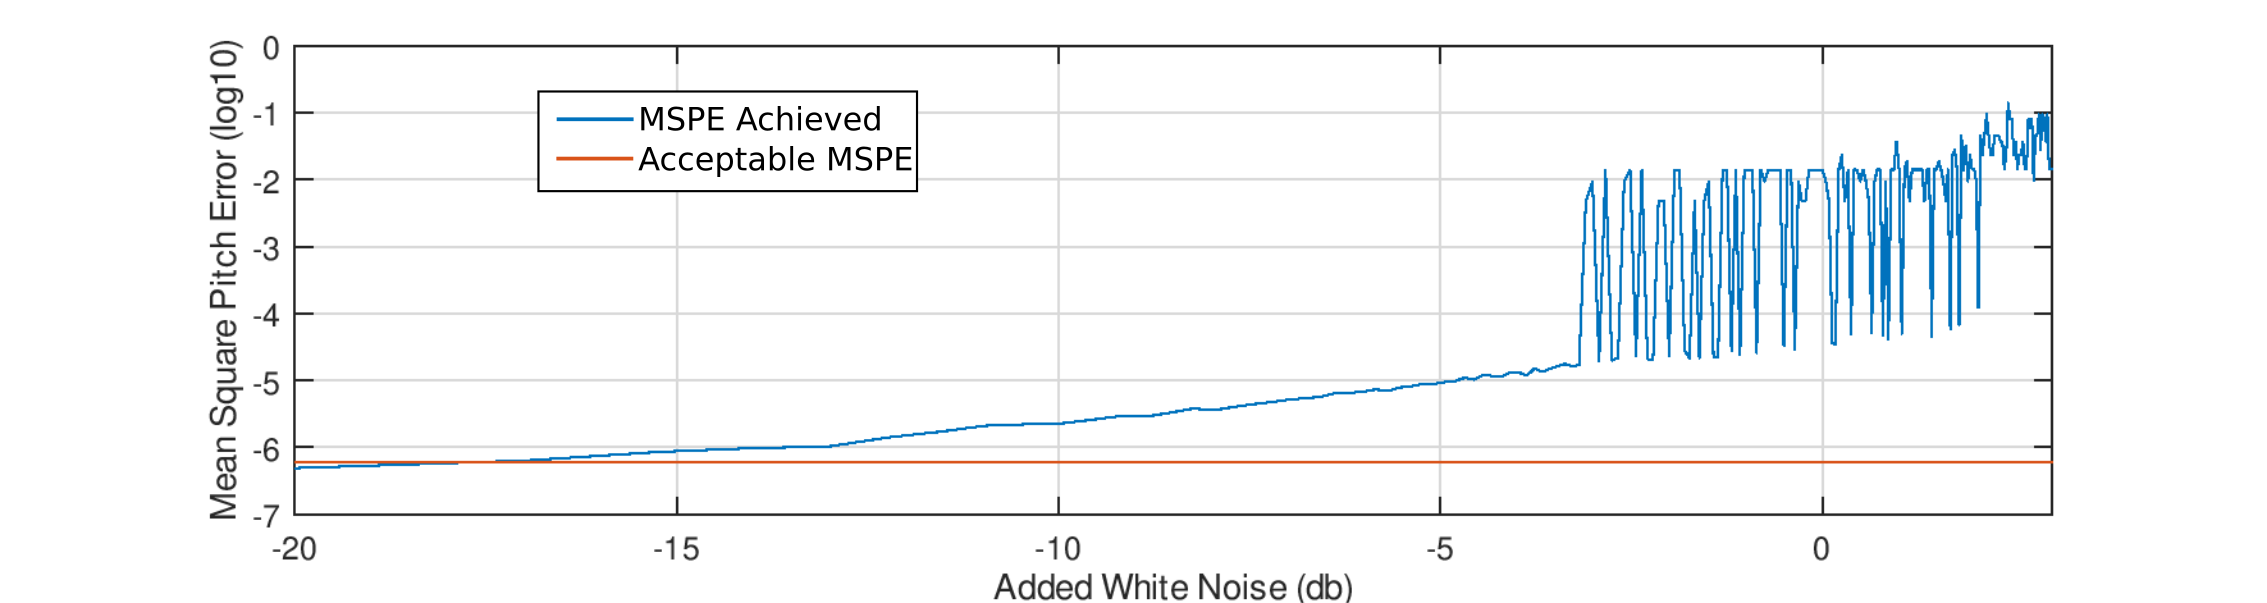
\includegraphics[width=\textwidth,trim={2.5cm 0mm 2.5cm 0mm},clip]
	{NoiseRobustnessAutoCorr}
	\caption{Autocorrelation Method Noise Robustness}
	\label{fig:NoiseRobustnessAutoCorr}
\end{figure}

\section{Pitch Corrector}

Because of time constraints, only the combination of the zero-crossing method and
the phase vocoder, as sub-modules, will be tested. This combination does also seem
like the most likely combination to produce the best results. This is because of
the results seen when testing the sub-modules individually and during the
development of the modules.

The first metric to test is the effectiveness metric. The goal is to produce a
number to say: ``The pitch corrector improves the pitch accuracy by X times''.
Figure \ref{fig:EffectivenessPVZCM} shows the pitch contour plot of the test
defined in the implementation chapter.

\begin{figure}[h]
	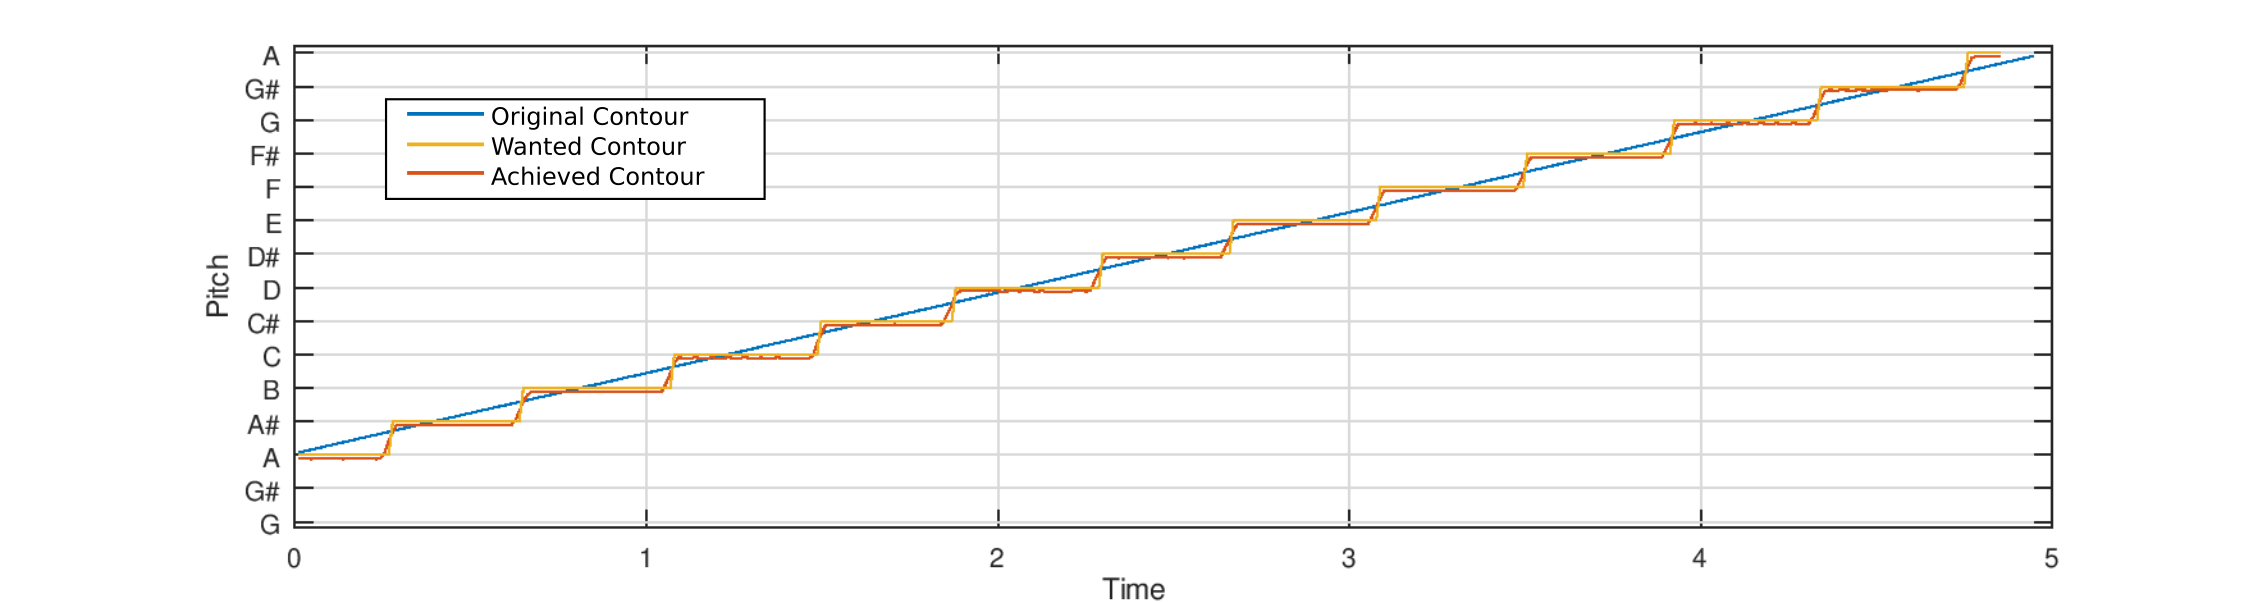
\includegraphics[width=\textwidth,trim={2.7cm 0mm 2.7cm 0mm},clip]
	{EffectivenessPVZCM}
	\caption{Visual Depiction of Effectiveness metric using Phase Vocoder and ZCM}
	\label{fig:EffectivenessPVZCM}
\end{figure}

The achieved pitch contour very narrowly follows the wanted pitch contour. The
mean squared pitch error before the correction was $0.59 \times 10^{-3}$, and
after the correction, $0.13 \times 10^{-3}$. This results in a pitch accuracy
improvement factor of 4.38.

Now that it is known by how much the system improves the pitch accuracy of the
signal, an indication of how much the signal is getting distorted by the system
needs to be acquired. This is given by the distortion metric defined in the
implementation chapter. To give some visual indication of what the distortion
metric is measuring, a logarithmically scaled spectrogram of the signal is shown
in figure \ref{fig:DistortionPVZCM}.

\begin{figure}[h]
	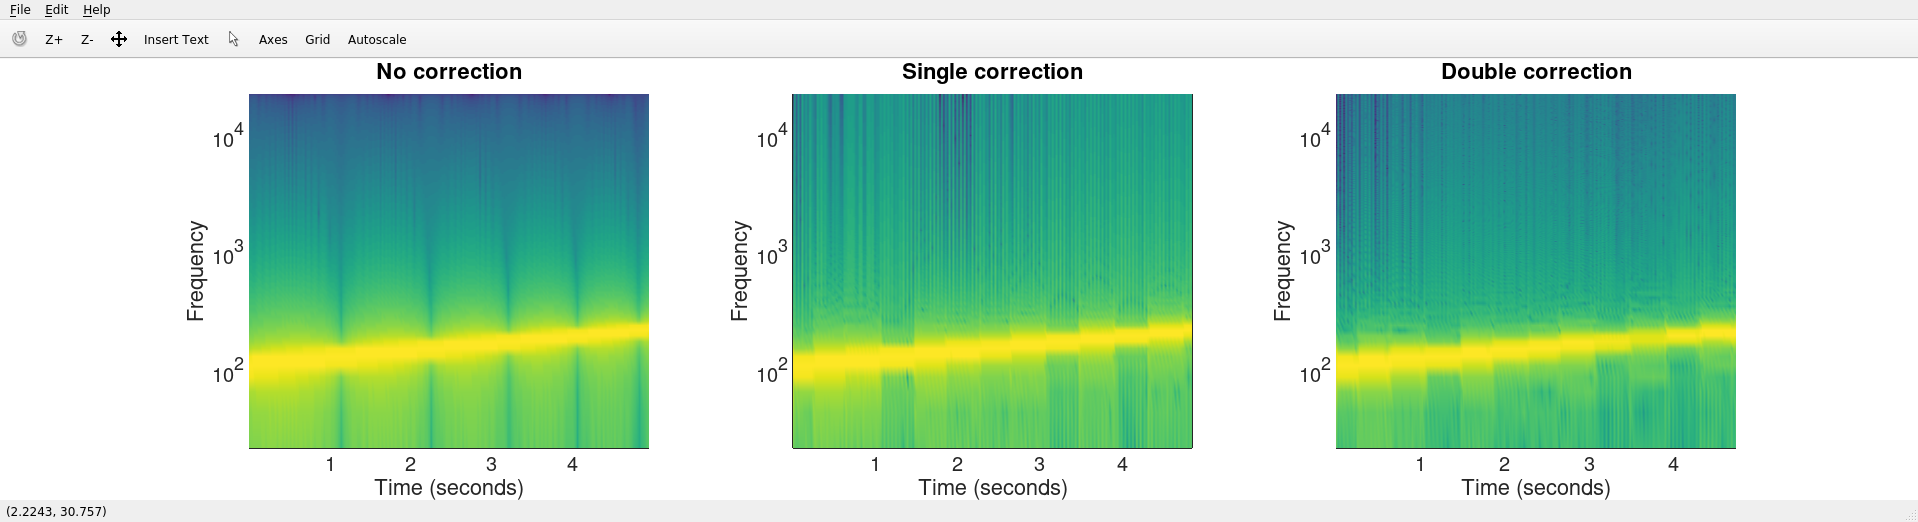
\includegraphics[width=\textwidth,trim={6cm 0.8cm 6cm 2.1cm},clip]
	{DistortionPVZCM}
	\caption{Visual Depiction of Distortion metric using Phase Vocoder and ZCM}
	\label{fig:DistortionPVZCM}
\end{figure}

This spectrogram shows the original signal on the left, followed by the result of
a single application and double application of the pitch correction effect. The
pitch correction system sees to introduce high frequency content on transitions
between notes. The second application of the effect, however, seems to slightly
remove the high frequency content on the transitions. This could be seen as a
positive effect and should be kept in mind when considering the distortion metric.

The result of the distortion metric is a quote of a ``percentage similar''. The
goal of a pitch corrector would be to maximise this similarity percentage. The
result of the distortion metric is 44\% similarity. Another, perhaps even more
meaningful, assessment of similarity may be to normalize the maximum value of the
autocorrelation between the first and second application of the correction effect,
not with the maximum value of the autocorrelation of the middle signal, but rather
the third. The result of this similarity quote is 61\%.


\chapter{Conclusions}
% !tex root = ../Thesis.tex

\section{Findings}

\color{red}
To do:
\begin{itemize}
	\item Summarise the thesis
	\item Does it work or not
\end{itemize}
\color{black}

\section{Recommendations}

\color{red}
To do:
\begin{itemize}
	\item Explain how I fucked up and what more can be done to make it better
\end{itemize}
\color{black}


\bibliography{references}{}
\bibliographystyle{ieeetr}
\addcontentsline{toc}{chapter}{References}

\chapter*{Appendix}
\setcounter{section}{0}
\renewcommand\thesection{\Alph{section})}
\addcontentsline{toc}{chapter}{Appendix}
\pagestyle{plain}

\section{Imperfect Tuning System Proof}

% !tex root = ../Thesis.tex

To prove* that no perfect tuning system exists, is equivalent to proving the
following proposition:

\begin{equation}\label{eq:GeneralProp}
	\nexists r \in \mathbb{R} \text{ s.t. }
	R \subseteq \{ r^n | n \in \mathbb{N}_0 \}
	\text{ where } R = \{ \frac{1}{1}, \frac{15}{16}, \frac{9}{8}, \frac{6}{5}, \dots \}
\end{equation}

R is the set of all the harmonic ratios required in the wanted tuning system. Only
two of these ratios, the most fundamental ratios in any tuning system, are
required for the proof. The octave interval, ratio 2/1, and the perfect fifth, ratio
3/2. The proof approach is a proof by contradiction.

Assume there exists:
\begin{equation}\label{eq:SpecificProp}
	r^n = \frac{2}{1} \text{ and } r^m = \frac{3}{2}
	\text{ s.t. }
	r \in \mathbb{R} \text{ and } n,m \in \mathbb{N}_0
\end{equation}

Taking the $\log_{2}$ of each equation in \ref{eq:SpecificProp} the following two
equations are obtained:

\begin{equation}\label{eq:1}
	\log_{2}(r) = \frac{\log_{2}(2)}{n}
\end{equation}
\begin{equation}\label{eq:2}
	\log_{2}(r) = \frac{\log_{2}(3) - \log_{2}(2)}{m}
\end{equation}

Equating equation \ref{eq:1} and equation \ref{eq:2} and simplifying, the following
equation is obtained:
\begin{equation}\label{eq:2}
	\log_{2}(3) = \frac{m+n}{n}
\end{equation}

Since both n and m are elements of $\mathbb{N}_0$, the RHS is rational.
The number $\log_{2}(3)$ is known to be irrational. This is a contradiction. Q.E.D.
\vfill
{\it *This proof was provided by Dr Neill Robertson of the UCT
Mathematics department}

\newpage

\section{Full AutoTalent Flow Diagram}
\vfill
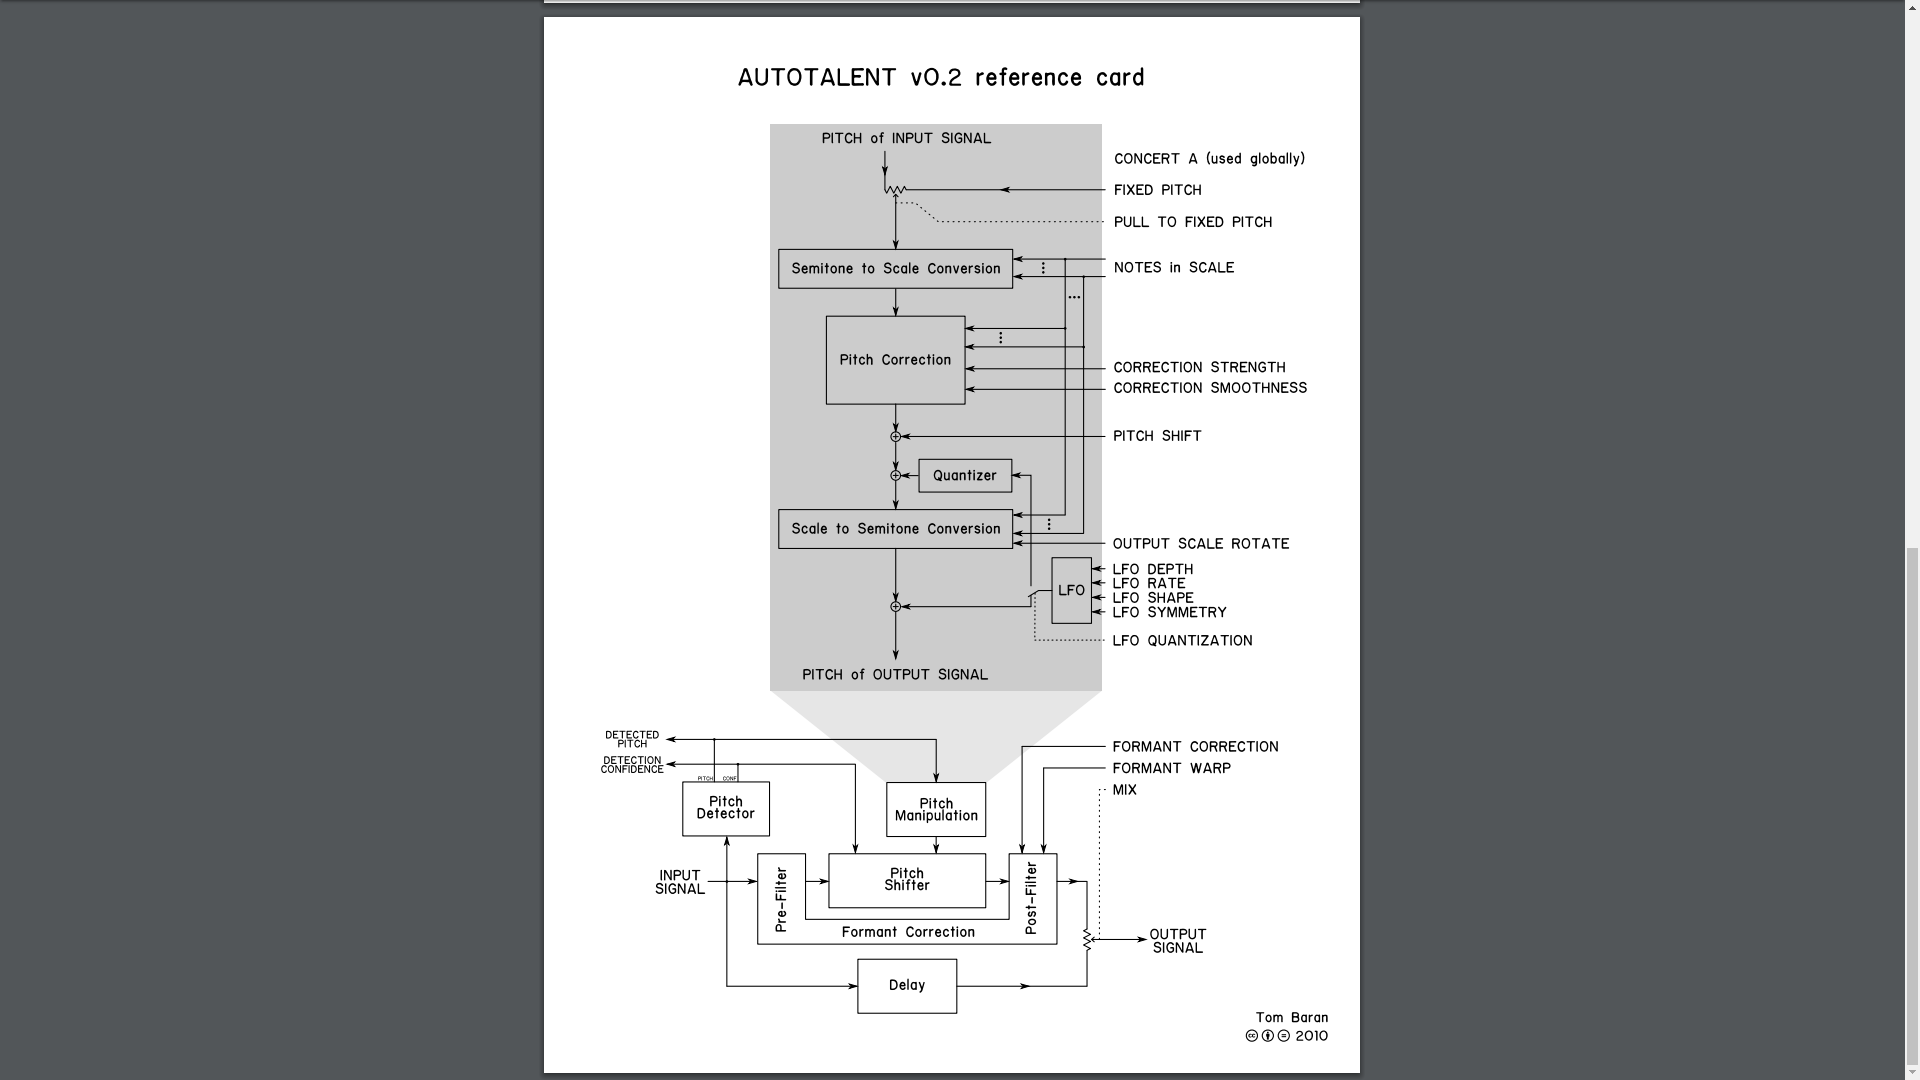
\includegraphics[width=\textwidth, trim={20cm 1cm 20cm 3.5cm},clip]
{AutoTalentFlowDiagram}
\vfill

\end{document}

%%%%%%%%%%%%%%%%%%%%%%%%%%%%%%%%%%%%%%%%%%%%%%%%%%%%%%%%%%%%%%%%%%%%%%%%%%%%%%%%%%
%%%%%%%%%%%%%%%%%%%%%%%%%%%%%%%% END OF DOCUMENT %%%%%%%%%%%%%%%%%%%%%%%%%%%%%%%%%
%%%%%%%%%%%%%%%%%%%%%%%%%%%%%%%%%%%%%%%%%%%%%%%%%%%%%%%%%%%%%%%%%%%%%%%%%%%%%%%%%%
